Establecimos como objetivo determinar enlaces submarinos en base al tiempo ZRTT de respuesta
Para ellos, como vimos, enviamos paquetes de control a universidades de otros continentes.

En esta secci\'on mostraremos los resultados obtenidos en la comunicaci\'on con 
Asia (MSU y Tsinghua), Europa (Oxford) y Ocean\'ia (Queensland), mostrando la ubicaci\'on en 
el mapa de los nodos m\'as importantes por los que se transmiten los paquetes y donde 
pueden verse los saltos intercontinentales que uno espera encontrar.

Luego mostraremos gr\'aficos de barras de IP en funci\'on de zscore con los umbrales que 
encontramos emp\'iricamente. Si el umbral es adecuado, \'unicamente los zscores de los 
enlaces submarinos estar\'an por encima del mismo.

Cabe aclarar que intentamos hacer uso de la herramienta www.geoiptool.com para orientarnos en 
el curso de las rutas y la mayoria de las veces lo que encontrabamos es que no tenian sentido las 
ubicaciones que nos proponia esta herramienta.

Afortunadamente capturamos los nombres de los hosts y la mayoria tiene indicios de ubicaci\'on en sus
nombres. Claro que no siempre encontramos hosts 'bien nombrados'.

Un ejemplo podr\'ia ser \emph{be2384.ccr21.\textbf{lpl}01.atlas.cogentco.com} con el c\'odigo IATA de 
Liverpool.

\subsection{MSU}

Veamos para Moscow State University (MSU), en Rusia:

Los resultados para los distintos hops pueden verse resumidos en la siguiente tabla.

~

\begin{tabular}{llll}
	\textit{\textbf{Ubicaci\'on}}	&	\textit{\textbf{IP}}	&	\textit{\textbf{RTT(media)}}	&	\textit{\textbf{ZScore}}	\\
	Buenos Aires	&	200.51.240.181	&	31.018	&	0.220	\\
	Buenos Aires (telef\'onica)	&	94.142.103.153	&	30.104	&	-0.265	\\
	Miami (telef\'onica)		&	94.142.123.22	&	164.933	&	\textcolor{red}{1.795}	\\
	Dallas (telef\'onica)		&	94.142.127.105	&	199.813	&	0.278	\\
	Dallas/Ft Worth (cogentco)	&	154.54.13.225	&	221.383	&	0.077	\\
	Dallas/Ft Worth (cogentco)	&	154.54.7.45	&	212.266	&	-0.389	\\
	Kansas (cogentco)		&	154.54.2.113	&	214.954	&	-0.210	\\
	Chicago (cogentco)		&	154.54.6.86	&	215.663	&	-0.240	\\
	Toronto (cogentco)		&	154.54.27.182	&	228.466	&	-0.056	\\
	Montreal (cogentco)	&	154.54.30.206	&	226.107	&	-0.286	\\
	Liverpool (cogentco)	&	154.54.44.138	&	294.383	&	\textbf{0.785}	\\
	Amsterdam (cogentco)	&	154.54.77.245	&	307.648	&	-0.049	\\
	Hamburgo (cogentco)	&	154.54.74.122	&	264.320	&	-0.908	\\
	Estocolmo (cogentco)	&	154.54.63.2	&	327.827	&	\textbf{0.713}	\\
	Helsinki (cogentco)		&	154.54.62.250	&	332.424	&	-0.181	\\
	Mosc\'u			&	149.6.58.42	&	333.589	&	-0.233	\\
	Mosc\'u (runnet)		&	194.85.40.229	&	525.315	&	\textcolor{red}{2.658}	\\
	Mosc\'u 			&	194.190.254.118	&	357.420	&	-2.798	\\
	Mosc\'u (runnet)		&	93.180.0.172	&	344.003	&	-0.454	\\
	Mosc\'u			&	188.44.33.1	&	346.421	&	-0.214 	\\
	Mosc\'u			&	188.44.50.103	&	347.007	&	-0.242	\\

\end{tabular}

~

Podemos ver que la ruta pasa de Am\'erica del Sur (BUE) a Am\'erica del Norte (MIA), luego de Canada en America del Norte (Montreal) a Europa (Liverpool) y por \'ultimo llega a Mosk\'u en Asia. En los dos primeros saltos, el ZScore es bastante alto, y por eso resalta en la tabla. 

\begin{figure}[H]
	\begin{center}
		  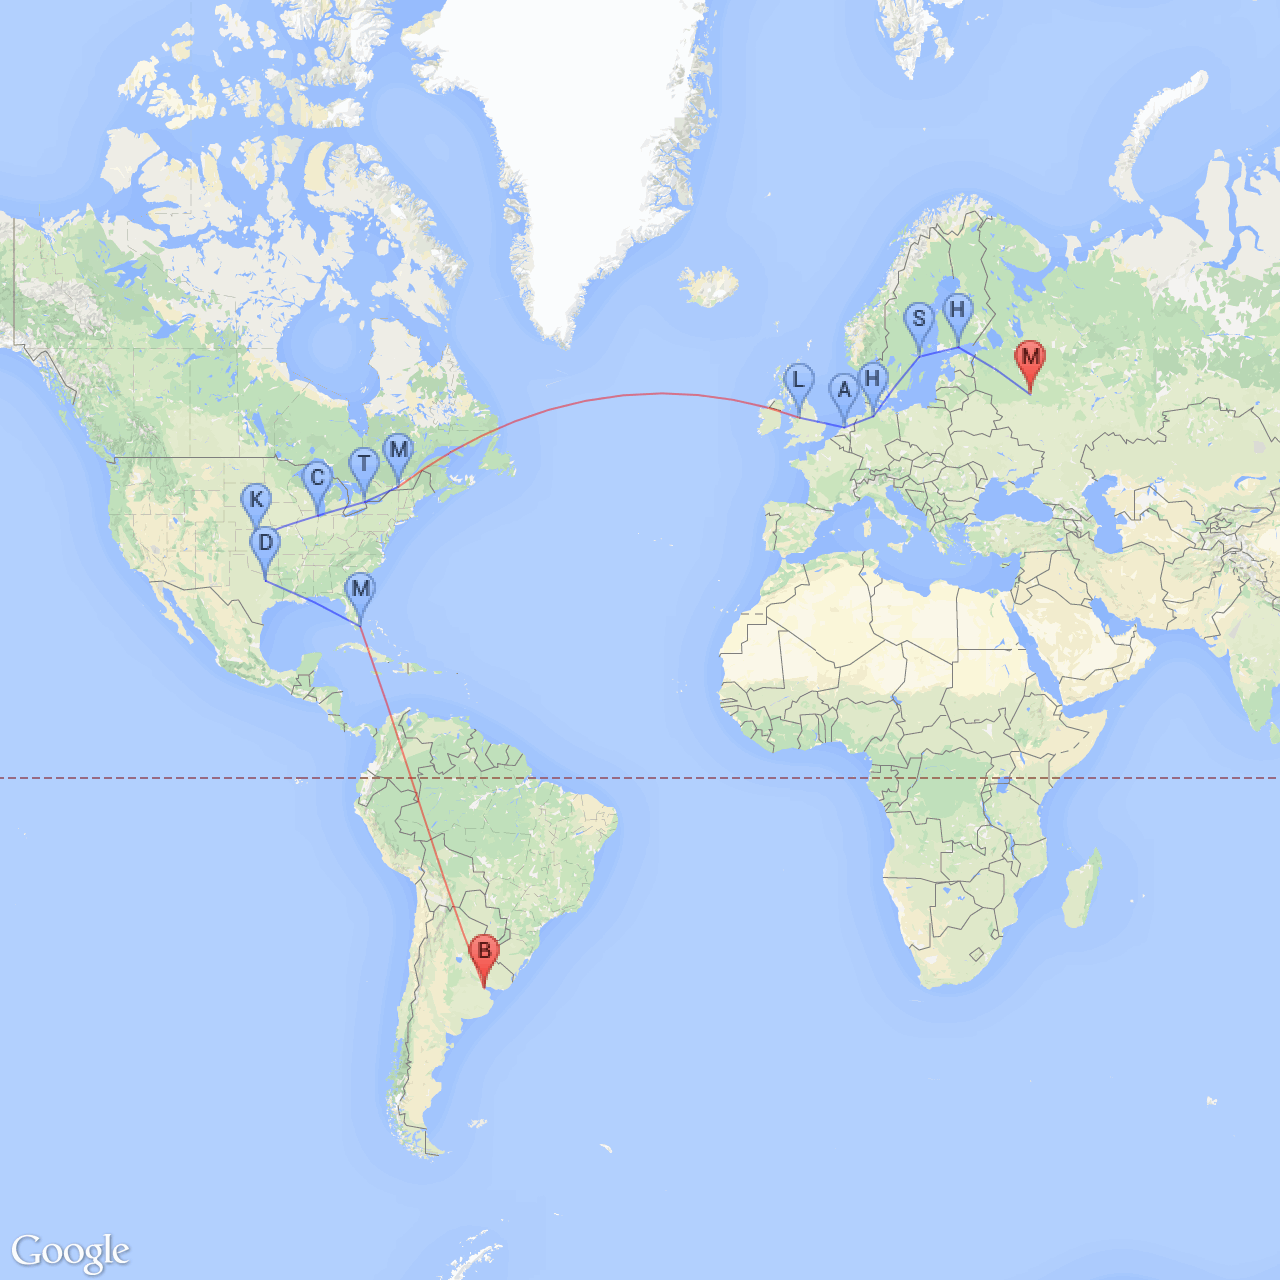
\includegraphics[scale=0.25]{../results/maps/MSU.png}
		  \caption{Mapa de la ruta atravesada para llegar a la universidad de Rusia}
	\end{center}
\end{figure}

\textcolor{red}{mas analisis y grafico de barra IP zscore + umbral}

\subsection{Tsinghua}

Para el caso de China, la ruta comienza por Estados Unidos como el caso anterior, pero en lugar de cruzar a Europa por el Este, los paquetes viajan por el pac\'ifico.
Veamos la siguiente tabla.

~

\begin{tabular}{llll}
	\textit{\textbf{Ubicaci\'on}}	&	\textit{\textbf{IP}}	&	\textit{\textbf{RTT(media)}}	&	\textit{\textbf{ZScore}}	\\
	Buenos Aires	&	200.51.240.156	&	31.907	&	0.259	\\
	Buenos Aires (telef\'onica)	&	84.16.9.233	&	30.095	&	-0.437	\\
	Miami (telef\'onica)		&	94.142.121.222	&	165.469	&	\textcolor{red}{2.396}	\\
	Miami (telef\'onica)		&	94.142.122.249	&	165.140	&	-0.407	\\
	Miami (telef\'onica)		&	84.16.12.238	&	167.934	&	-0.342	\\
	Miami 			&	63.243.152.45	&	164.176	&	-0.478	\\
	Ashburn			&	66.198.154.177	&	265.945	&	textbf{1.702}	\\
	Dallas			&	66.198.154.118	&	254.661	&	-0.633	\\
	Dallas			&	66.110.56.6	&	267.287	&	-0.139	\\
	Los-Angeles		&	66.110.57.82	&	256.103	&	-0.631	\\
	66.110.59.182		&	66.110.59.182	&	257.170	&	-0.378	\\
	Beijing			&	101.4.117.213	&	428.694	&	\textcolor{red}{3.143}	\\
	Beijing			&	101.4.117.97	&	428.055	&	-0.413	\\
	Beijing			&	101.4.116.146	&	424.990	&	-0.463	\\
	Beijing			&	101.4.118.78	&	427.001	&	-0.358	\\
	Beijing			&	202.112.38.10	&	425.663	&	-0.428	\\
	Beijing			&	118.229.4.66	&	425.672	&	-0.400	\\
	Beijing			&	118.229.4.34	&	438.217	&	-0.141	\\
	Beijing			&	118.229.2.74	&	430.018	&	-0.569	\\
	Beijing			&	118.229.2.69	&	425.922	&	-0.485	\\
	Beijing			&	118.229.8.6	&	427.147	&	-0.375	\\
	Beijing (Tsinghua)		&	166.111.4.100	&	426.084	&	-0.422	\\

\end{tabular}

~

\begin{figure}[H]
	\begin{center}
		  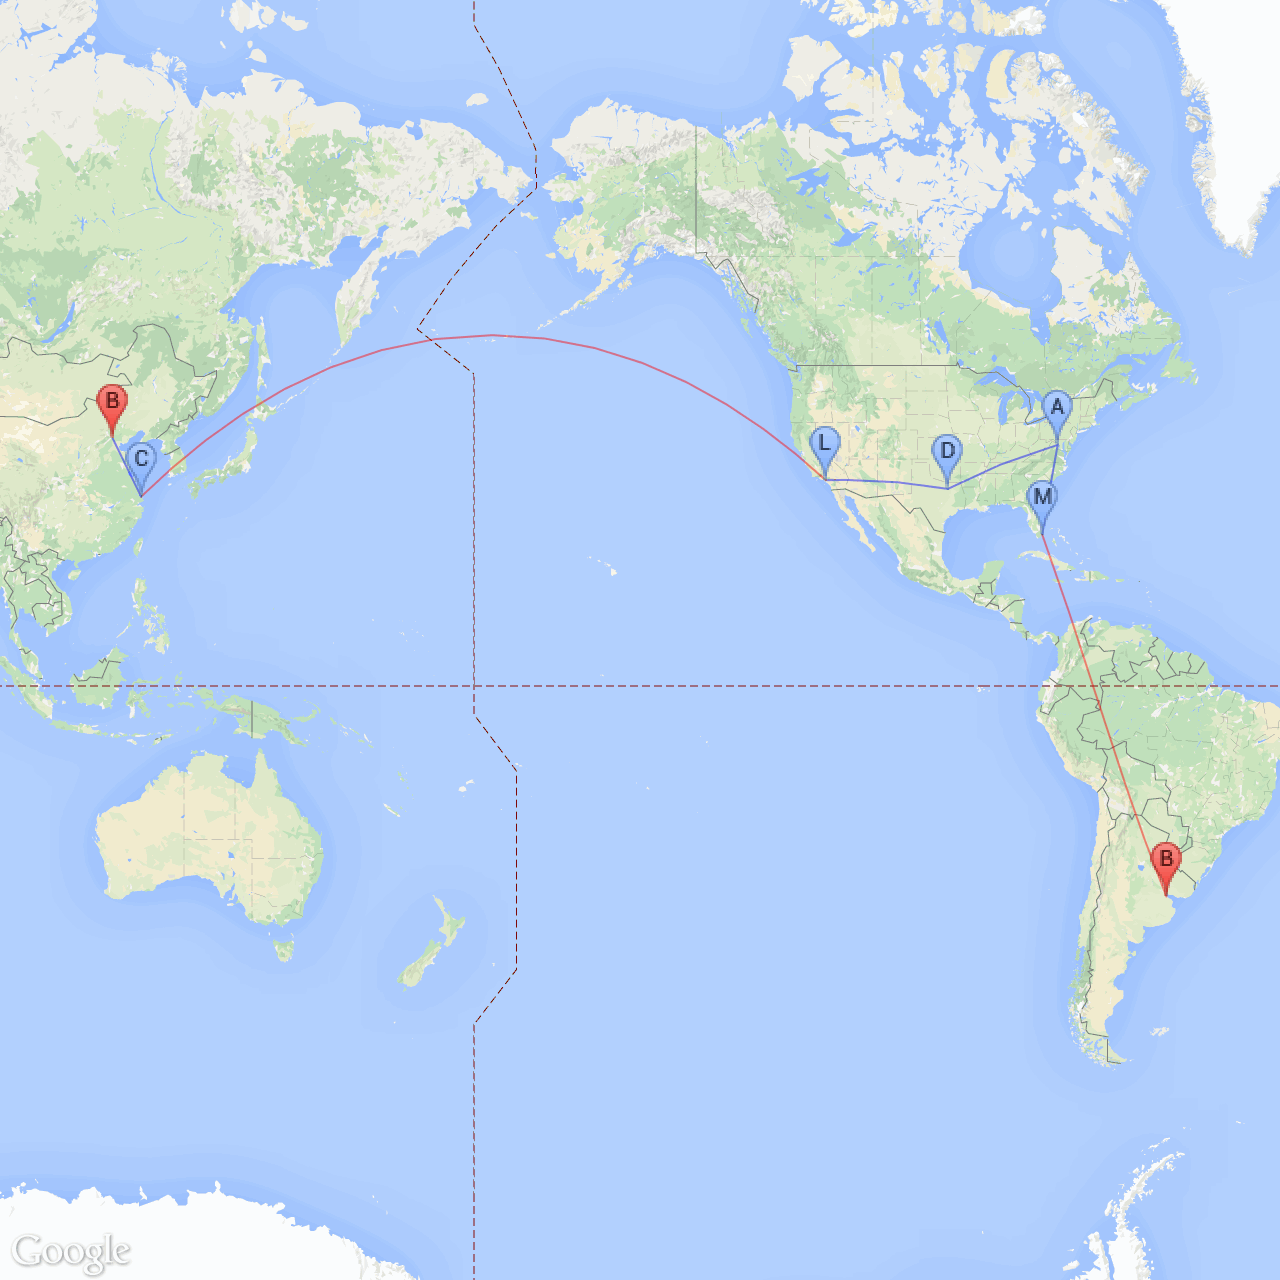
\includegraphics[scale=0.25]{../results/maps/Tsinghua.png}
		  \caption{Mapa de la ruta atravesada para llegar a la universidad de China}
	\end{center}
\end{figure}

\textcolor{red}{mas analisis y grafico de barra IP zscore + umbral}

\subsection{Oxford}

~

\begin{tabular}{llll}
	\textit{\textbf{Ubicaci\'on}}	&	\textit{\textbf{IP}}	&	\textit{\textbf{RTT(media)}}	&	\textit{\textbf{ZScore}}	\\
	Buenos Aires			&	200.51.240.181	&	37.154	&	0.426	\\
	Buenos Aires (telef\'onica)	&	84.16.9.233	&	51.008	&	-0.009	\\
	Miami (telef\'onica)		&	5.53.5.138	&	210.915	&	2.722	\\
	Miami (telef\'onica)		&	94.142.123.5	&	174.734	&	-0.945	\\
	Miami (as6453)			&	63.243.152.45	&	175.240	&	-0.259	\\
	Ashburn (as6453)		&	66.198.154.177	&	293.857	&	1.950	\\
	Ashburn (as6453)		&	216.6.87.1	&	286.600	&	-0.404	\\
	Newark (as6453)			&	216.6.87.138	&	277.667	&	-0.435	\\
	Newark (as6453)			&	66.198.70.1	&	307.315	&	0.286	\\
	London (as6453)			&	66.198.70.26	&	403.133	&	1.523	\\
	London (as6453)			&	80.231.130.42	&	298.757	&	-2.220	\\
	195.219.100.82			&	195.219.100.82	&	285.687	-0.513	\\
	ae29.londpg-sbr1.ja.net	146.97.33.2	&	289.063	&	-0.205	\\
	ae21.read-rbr3.ja.net	146.97.37.206	&	291.484	&	-0.223	\\
	ae1.read-rbr2.ja.net	193.63.108.129	&	281.783	&	-0.450	\\
	ae2.oxfo-rbr2.ja.net	193.63.108.134	&	294.226	&	-0.036	\\
	Oxford-University-2.ja.net	193.63.109.114	&	289.814	&	-0.351	\\
	csurb.backbone.ox.ac.uk	192.76.21.21	&	280.879	&	-0.435	\\
	bmusb.backbone.ox.ac.uk	192.76.22.201	&	282.251	&	-0.243	\\
	bmus-lompi1.sdc.ox.ac.uk	192.76.32.66	&	286.466	&	-0.190	\\
	aurochs-web-155.nsms.ox.ac.uk	129.67.242.155	&	301.388	&	0.011	\\

\end{tabular}

~

\begin{figure}[H]
	\begin{center}
		  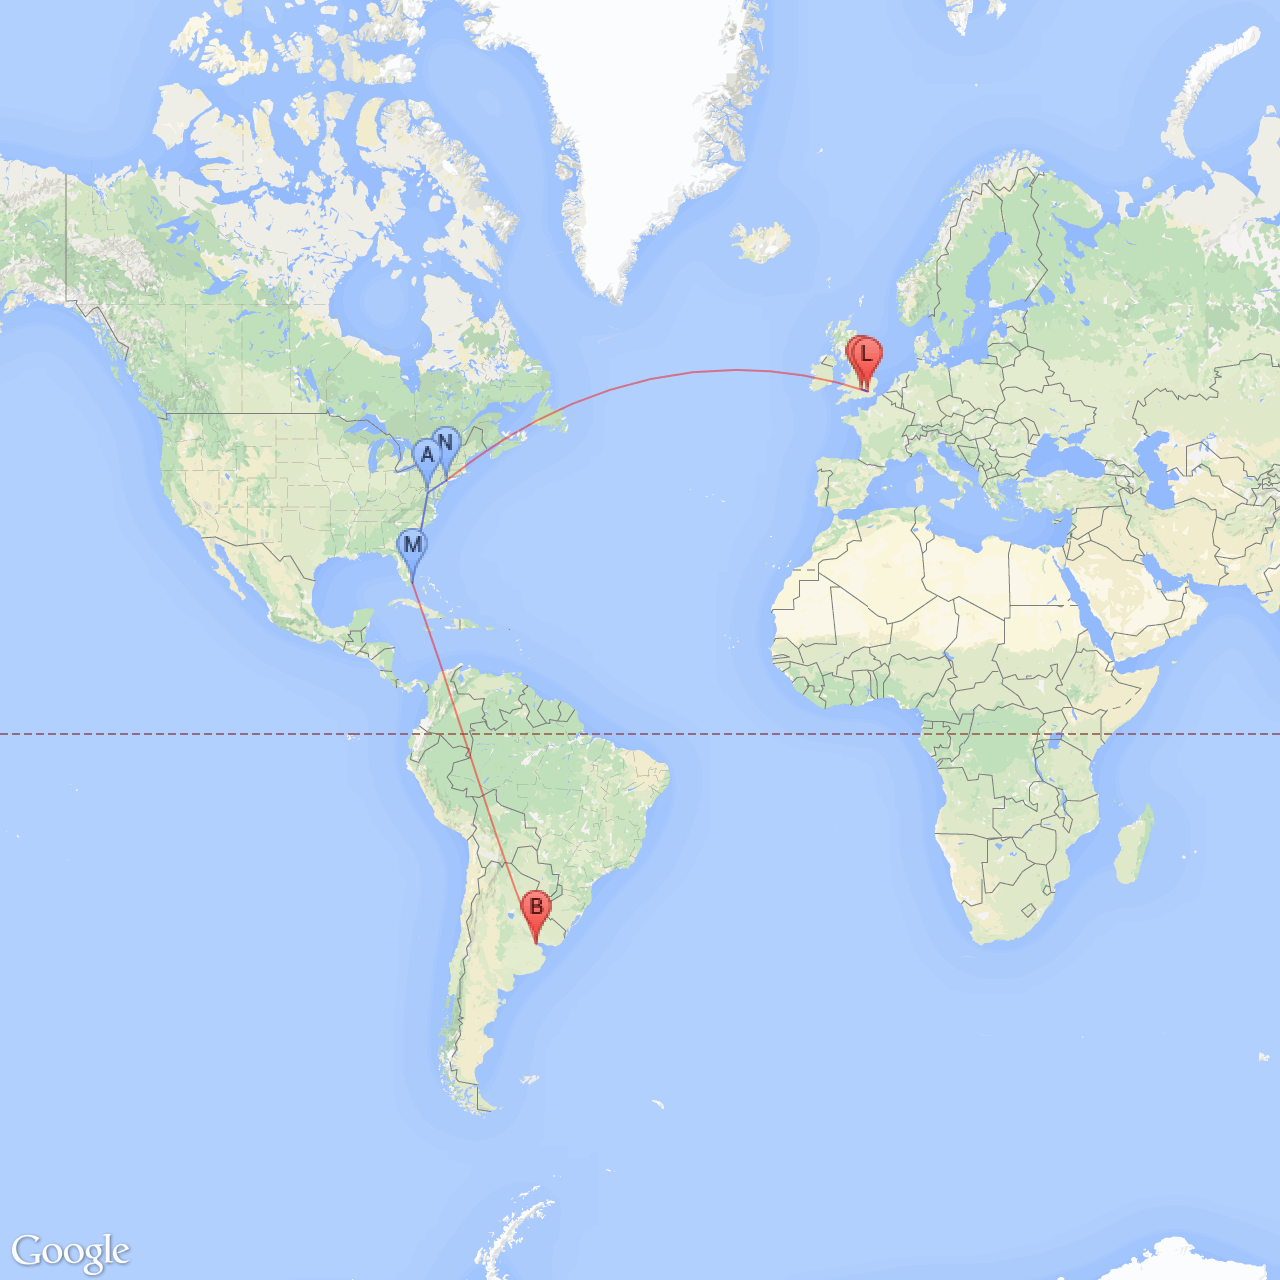
\includegraphics[scale=0.25]{../results/maps/Oxford.png}
		  \caption{Mapa de la ruta atravesada para llegar a la universidad de Inglaterra}
	\end{center}
\end{figure}

\textcolor{red}{mas analisis y grafico de barra IP zscore + umbral}

\subsection{Queensland}

~

\begin{tabular}{llll}
	\textit{\textbf{Ubicaci\'on}}	&	\textit{\textbf{IP}}	&	\textit{\textbf{RTT(media)}}	&	\textit{\textbf{ZScore}}	\\
	Buenos Aires	&	200.51.240.156	&	31.896	&		0.110	\\
	et-7-0-0-0-grtbuecu1.red.telefonica-wholesale.net	(84.16.9.233	&	30.748	&	-0.399	\\
	\\	Xe9-0-6-0-grtmiabr3.red.telefonica-wholesale.net	(94.142.123.14	&	165.811	&	1.700	\\
	213.140.49.13	(213.140.49.13	&	230.069	0.609	\\
	xe-3-1-1.mpr1.pao1.us.above.net	(64.125.13.113	&	229.511	&	-0.390	\\
	208.185.52.74.available.above.net	(208.185.52.74	&	392.486	&	2.131	\\
	xe-1-2-1.pe2.brwy.nsw.aarnet.net.au	(202.158.194.176	&	391.129	&	-0.403	\\
	ae9.bb1.a.syd.aarnet.net.au	(113.197.15.57	&	514.913	&	1.527	\\
	so-0-1-0.bb1.b.bne.aarnet.net.au	(202.158.194.54	&	407.555	&	-2.037	\\
	ge-0-0-0.bb1.a.bne.aarnet.net.au	(202.158.194.213	&	394.376	&	-0.585	\\
	tengigabitethernet2-1.er2.uq.cpe.aarnet.net.au	(202.158.209.3	&	394.951	&	-0.373	\\
	gw2.er2.uq.cpe.aarnet.net.au	(113.197.8.34	&	391.479	&	-0.435	\\
	uq-se1-uq-gw1.router.uq.edu.au	(130.102.159.1	&	392.041	&	-0.373	\\
	zeus-uqse1.router.uq.edu.au	(130.102.0.242	&	401.994	&	-0.228	\\
	a82-28.nat.uq.edu.au	(130.102.82.28	&	403.280	&	-0.362	\\
	wsa-www.soe.uq.edu.au	(130.102.131.70	&	396.128	&	-0.492	\\
\end{tabular}

~

\end{tabular}

~

\begin{figure}[H]
	\begin{center}
		  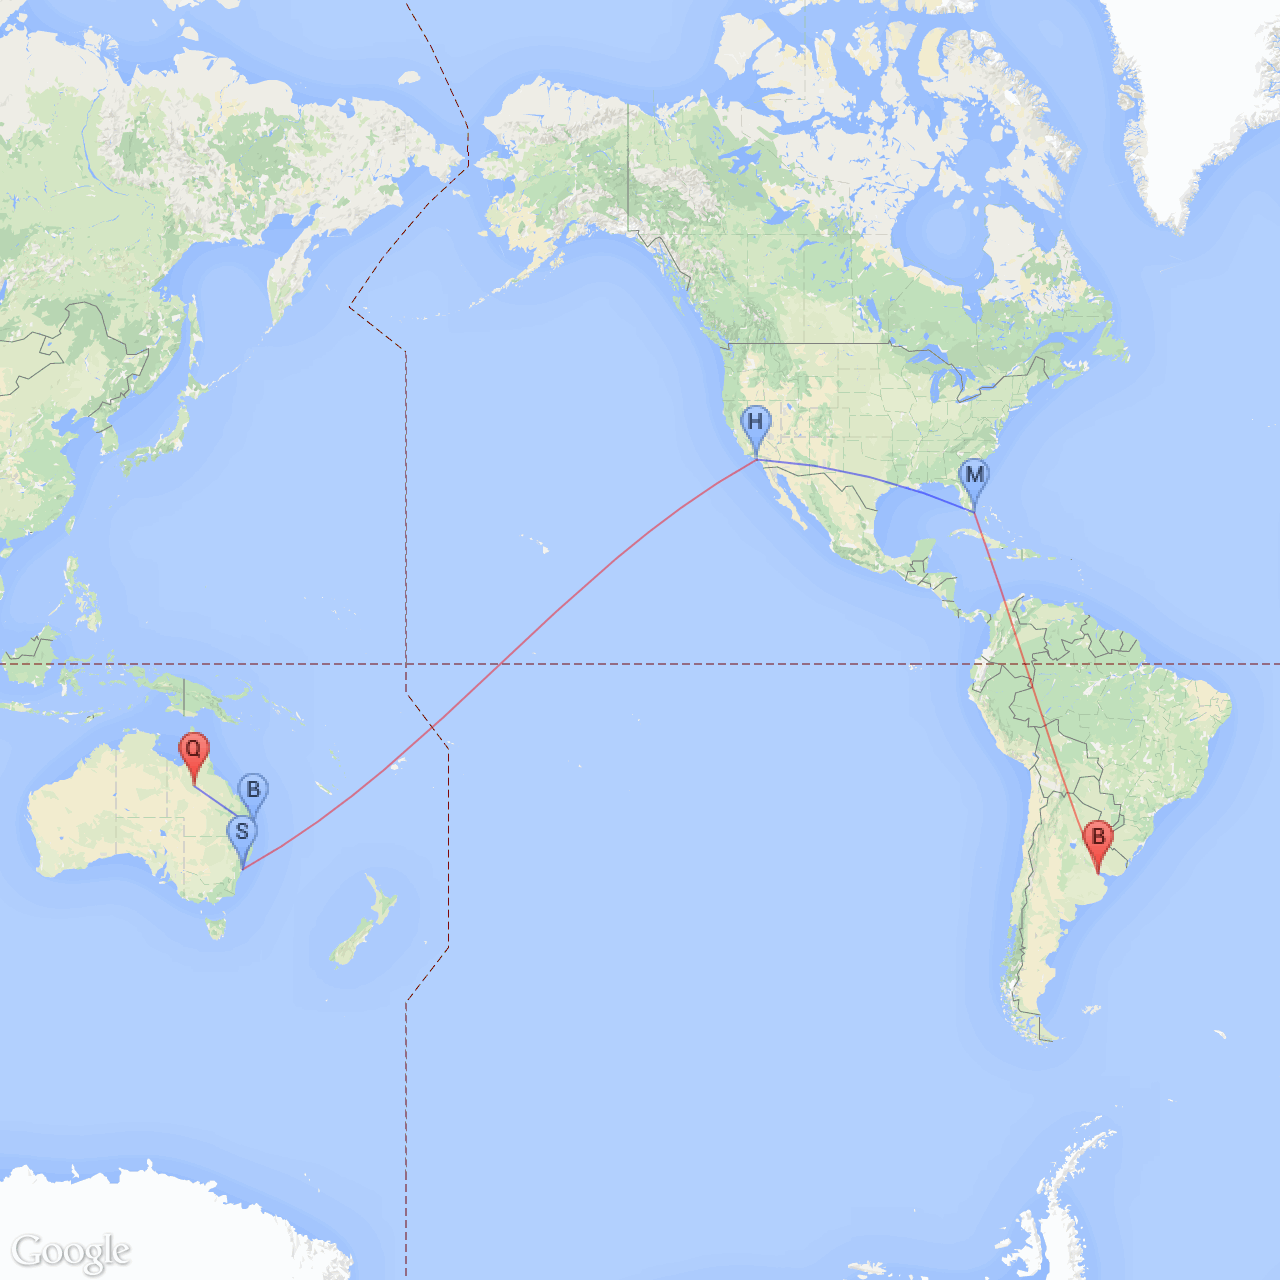
\includegraphics[scale=0.25]{../results/maps/Queensland.png}
		  \caption{Mapa de la ruta atravesada para llegar a la universidad de Australia}
	\end{center}
\end{figure}

\textcolor{red}{mas analisis y grafico de barra IP zscore + umbral}
